%%%%%%%%%%%%%%%%%%%%%%%%%%%%%%%%%%%%%%%%%
% University/School Laboratory Report
% LaTeX Template
% Version 3.1 (25/3/14)
%
% This template has been downloaded from:
% http://www.LaTeXTemplates.com
%
% Original author:
% Linux and Unix Users Group at Virginia Tech Wiki 
% (https://vtluug.org/wiki/Example_LaTeX_chem_lab_report)
%
% License:
% CC BY-NC-SA 3.0 (http://creativecommons.org/licenses/by-nc-sa/3.0/)
%
%%%%%%%%%%%%%%%%%%%%%%%%%%%%%%%%%%%%%%%%%

%----------------------------------------------------------------------------------------
%	PACKAGES AND DOCUMENT CONFIGURATIONS
%----------------------------------------------------------------------------------------

\documentclass{article}
\usepackage[margin=1in]{geometry}
\usepackage{float}
\usepackage{multicol}
\usepackage{textcomp}
\usepackage{caption}
\usepackage{gensymb}
\usepackage{circuitikz}
\usepackage{siunitx} % Provides the \SI{}{} and \si{} command for typesetting SI units
\usepackage{graphicx} % Required for the inclusion of images

\usepackage{amsmath} % Required for some math elements 

%\setlength\parindent{0pt} % Removes all indentation from paragraphs

\renewcommand{\labelenumi}{\alph{enumi}.} % Make numbering in the enumerate environment by letter rather than number (e.g. section 6)
\usepackage{tabulary}
%\usepackage{times} % Uncomment to use the Times New Roman font

%----------------------------------------------------------------------------------------
%	DOCUMENT INFORMATION
%----------------------------------------------------------------------------------------
\title{\vspace{6cm}Laser Pinball \\ Final Report \\\vspace{1cm} MIT 6.111} % Title

\author{Weston Braun, Pauline Varley, and Jake Isenhart} % Author name

\date{December 10, 2014} % Date for the report\

\begin{document}

\maketitle % Insert the title, author and date
\vspace{8cm}
\begin{center}
\begin{tabular}{l r}
Professor: & Gim P. Hom \\
Term: & Fall 2014
\end{tabular}
\end{center}

\pagebreak

%----------------------------------------------------------------------------------------
%	INTRODUCTION
%----------------------------------------------------------------------------------------

\section{Introduction} \label{intro}

For our final project, we wanted to create a pinball-like arcade game on an FPGA that would be displayed on a wall by an RGB laser projector. The system would allow the user to reconfigure the gameboard by recognizing colored objects on a wall; each color would correspond to a different game object, and the objects would appear in-game in the location in which they were placed on the wall. This project was motivated by a desire to use technology for enjoyment rather than academics; while discussing what we might want to build for our final project we found that, over the course of our MIT educations, we hadn't had much of an opportunity to just play around with tech in the way we do outside of class. We wanted a project that we could get excited about and a project that we could share with our peers without too much explanation—a laser-projected game is, undoubtedly, very cool and fits that criteria to a tee.

In our implementation of the proposed design we encountered a series of unexpected difficulties that prevented us from finishing all planned elements of the project. Interfacing with the camera module was particularly difficult (see sections XXX and XXX), and implementing a physics engine in Verilog so complex that we decided to scrap the initial architecture entirely and build the project on Beta processors that we implemented using Verilog (section XXX). These challenges will be discussed further in section 4.

We did, however, accomplish several exciting things: design and implementation of a "µBeta" processor; functional image recognition that can detect red, green, and blue objects; physics emulation written entirely in assembly; and a laser-projected gameboard with paddles that can be controlled with an NES controller.  These successes will be further discussed in sections 3 and 4.


%----------------------------------------------------------------------------------------
%	SUMMARY
%----------------------------------------------------------------------------------------
\section{Summary} \label{summary}

\begin{figure}[H]
\begin{center}
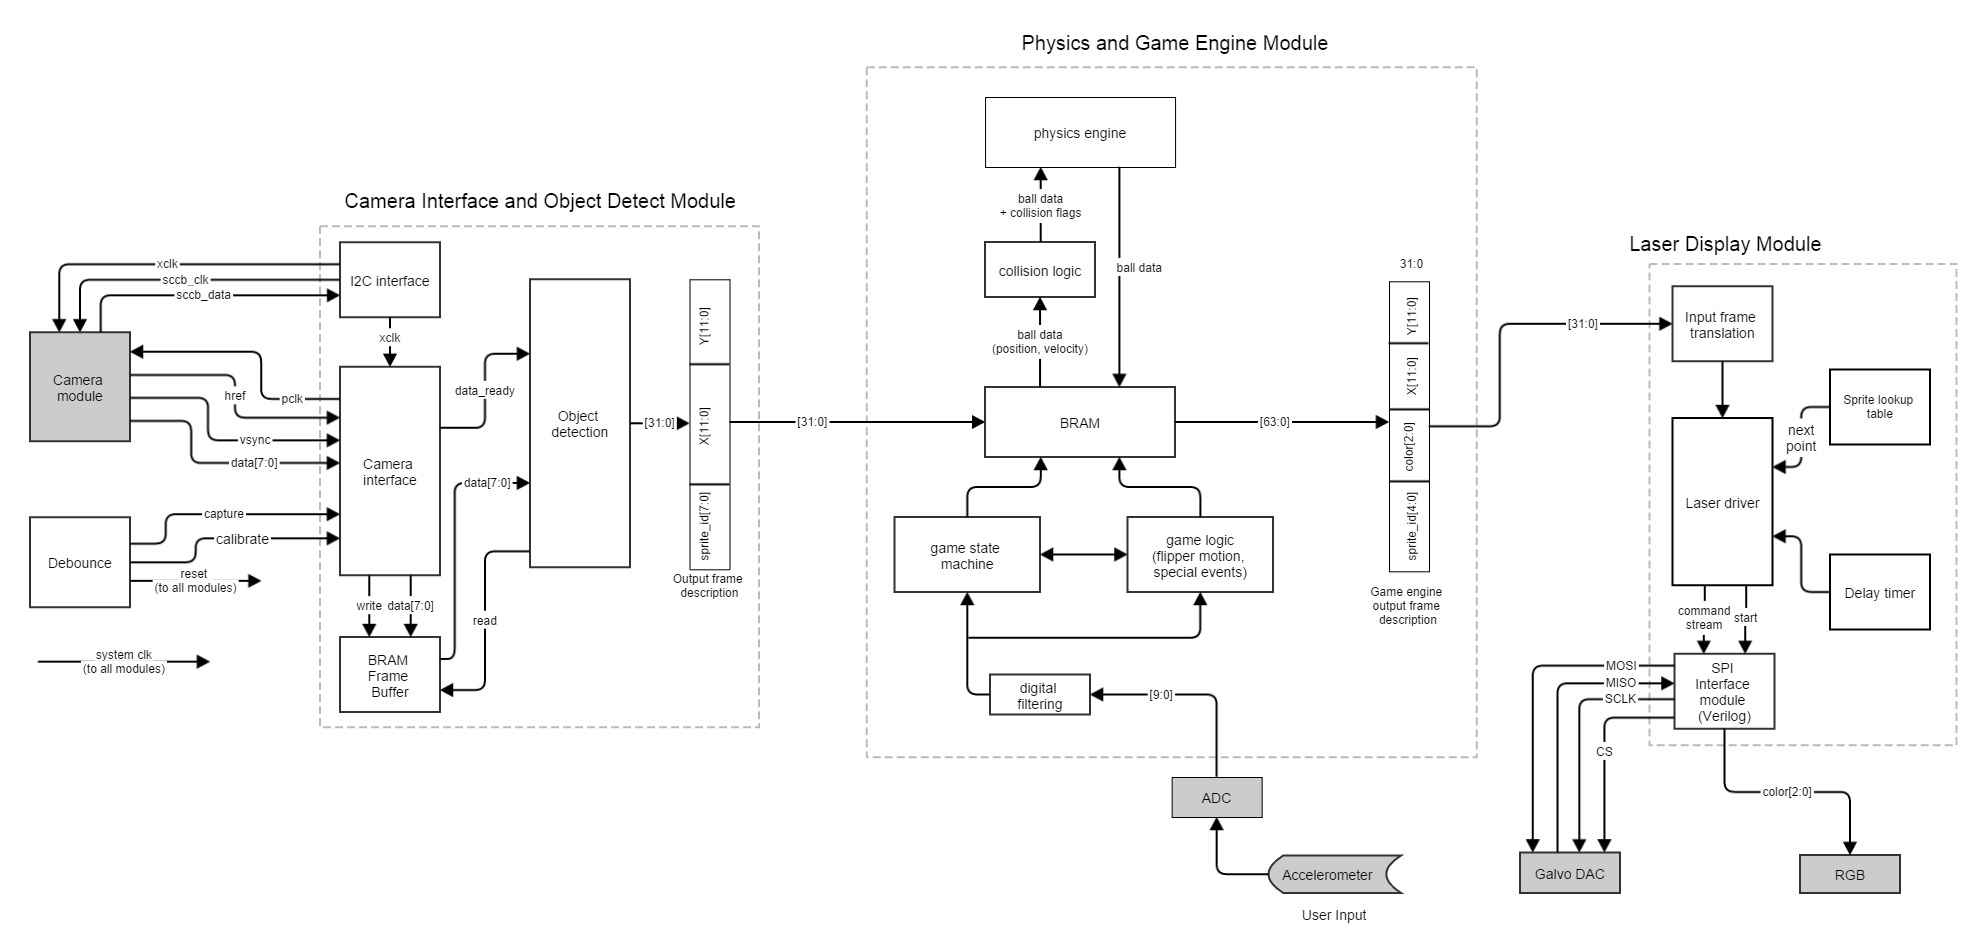
\includegraphics[width=\textwidth]{block_all} 
\caption{High-level system diagram. Each module will be explained in greater depth later in this report, and a full system diagram is included in the appendix.}
\end{center}
\end{figure}

Laser pinball was implemented as three discrete systems: a vision processing and object detect module, a physics and game engine, and a laser display controller.\footnote{Weston was responsible for the vision processing module; Jake and Pauline were primarily responsible for the physics engine and laser controller, respectively, but collaborated heavily on both. Weston also designed the external hardware interface and brought up the Beta processors.}  Though we originally planned on implementing the system entirely in Verilog, we realized about halfway through that the complexity of both the physics engine and the laser controller would be better suited to implementation on a microcontroller with a higher level of abstraction from the hardware. Since a Verilog implementation of the Beta processor already existed (to some degree—the bringup of the Beta will be discussed further in section SECTION NUMBER HERE), we decided to restructure both modules as assembly language code running on two separate Beta processors communicating via a shared memory interface. Despite this, the overall architecture of the system remained much the same.

The vision processing module takes input from an OV7670 camera, detects objects of three colors (one red, one green, and one blue), and outputs the corresponding sprite IDs and locations to the physics Beta processor over a shared memory interface.

%----------------------------------------------------------------------------------------
%	MODULES
%----------------------------------------------------------------------------------------

\section{Modules} \label{modules}
\subsection{Vision Processing and Image Recognition} \label{vp}

\begin{figure}[H]
\begin{center}
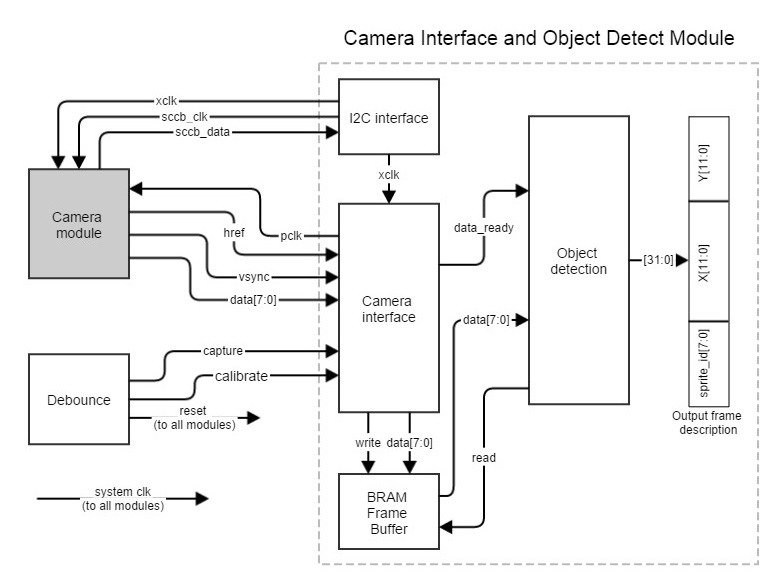
\includegraphics[width=0.75\textwidth]{camera} 
\caption{The camera interface module.}
\end{center}
\end{figure}

\subsubsection{The OV7670 Camera} \label{cameraintro}

The OV7670 camera was chosen because of its low cost and small size, allowing it to be mounted inside the laser projector case. The camera has an 8-bit output data bus, vertical (VSYNC) and horizontal (HREF) sync pins, and an output clock, and outputs 16-bit color over a 640x480 frame. The camera's output clock is internally generated by the camera from an input clock and is the same frequency as the input clock, but with different phasing. This required the crossing of clock domains within the FPGA. The camera outputs 8-bit wide sections of 16-bit wide pixels at twice the pixel clock frequency. An FSM was written in Verilog to synchronize the data capture of the camera with the start of the frame in order to capture a complete image. The frame starts on the falling edge of VSYNC and each line starts on the falling edge of HREF.

 Data captured from the camera was scaled down to 9-bit color and 240x240 pixels and stored in a dual port memory, which acted as a buffer to allow the crossing of clock domains. The down-sampling of color and resolution were due to constraints on the amount of BRAM within the FPGA and 9-bit resolution was used as the BRAM blocks have an input width of 9 bits: a byte plus a 9th bit storing a parity check value. We used this 9th bit to store additional color data. 
Unfortunately, the OV7670 camera has a quite complicated setup routine. The camera by default outputs YCrCb data instead of RGB. Additionally, the color balance is quite off to the point of red and green showing up reversed. The OV7670 camera contains a configuration interface called SCCB, which is essentially a royalty-free version of I2C and is I2C compatible. An open-source I2C core from the OpenCores project and licensed under the BSD license was used for I2C configuration. The core uses a Wishbone interface, which is an open source parallel bus standard. A Verilog FSM wrapper was written for the core to handle the Wishbone interface and an additional FSM was created to send configuration commands to the OV7670 camera from a ROM.

After image capture, the stored image was output to VGA using the Chrontel CH7301C DVI IC on the FPGA development board. This IC also required configuration over an I2C interface to be put in VGA pass-through mode. A version of the FSM used for camera configuration was reused to configure the Chrontel chip. 24-bit color is sent to the CH7301C through a 12-bit interface operating at twice the pixel clock by sending 12 bits at a time on each rising clock. A modified version of the VGA drive module from 6.111 lab 3 was taken to generate hsync and vsync signals for a 640x480 image at the faster pixel clock required by the CH7301C and to generate a pixel address to recall the stored image. A Verilog module was written to take 24-bit pixels and drive the 12-bit bus of the CH7301C.
	
\subsubsection{Image Recognition} \label{imagerec}

The goal of image recognition for the project was to recognize red, green, and blue game piece objects on a white background. As the game piece objects were to be small compared to the frame and were all primary colors, several simplifications could be made to the image processing process.

First, instead of calculating the mass of a single color, the image could be segmented into small sections, and a color classifier could be applied for each color that needed to be detected. The section of the image that had the the highest value for a given classifier was then detected as the center of a color block. 

The second simplification that could be made was in the classification of colors. Traditionally, the image is converted to the HSV color-space for classification. However, this process is computationally complex as it is not a linear mapping and requires the use of division, which is difficult to implement on an FPGA. Due to the low color resolution of the stored image and the need to only detect primary colors, a classifier was created that would directly translate an RGB color value into a set of color classifiers for red, green, and blue. This classifier would also have to reject mixtures of colors, such as white.
The classifier that was decided on for image recognition for each primary color was the value of the desired color minus the value of one of the other colors, multiplied by its value minus the other color. For red, this classifier would be $(red-green)\cdot(red-blue)$. This classifier worked well in distinguishing the colored game objects on a white wall. For processing, the image was split into 3600 squares of 16 pixels each. The 16 pixels in each block were averaged to remove noise and then run through the classifier. The three blocks that had the highest classifier values for red, green, and blue respectively were decided to be the coordinates of the detected objects. 

Image processing was implemented using a Verilog FSM that was triggered by a button on the FPGA board. Data was acquired from the read port of the dual port ram that the camera data was stored in, allowing the user to press a button to see live video from the camera, release the button to capture the frame, and then press a second button to analyze that particular frame. Once the frame was analyzed, a sprite was overlaid onto the stored image at the location of three detected color objects so that the user could confirm that the correct objects were recognized.

 Additionally, the location of each object was written into the memory space of the physics engine beta through the shared memory interface along with a done flag. 
 
\section{Physics and Game Engine} \label{physics}
\subsection{The NES Controller}

\section{Laser Controller} \label{laser}

\begin{figure}[H]
\begin{center}
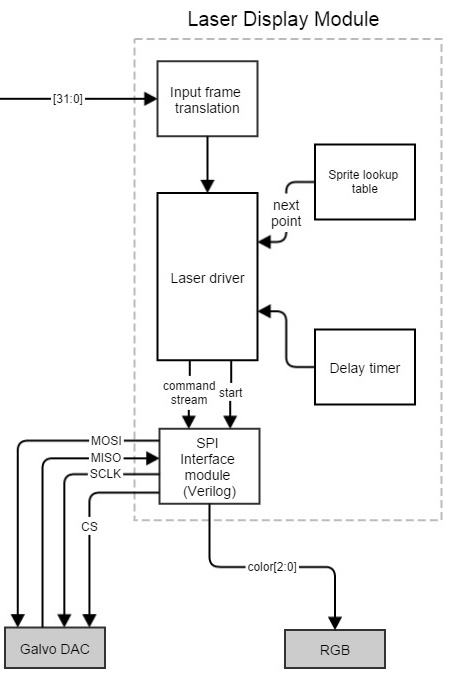
\includegraphics[width=0.5\textwidth]{laser}
\caption{The block diagram for the laser display module. Unless noted, all blocks were designed in Beta assembly language.}
\end{center}
\end{figure}

The laser display module was implemented primarily on a Beta processor, with the exception of the SPI interface module, which was implemented in Verilog as a simple state machine. The SPI module was then treated as a memory-mapped I/O device accessible by the laser Beta. Each frame, the laser Beta received form the physics Beta a series of one-word (32-bit) sprite descriptions detailing the ID of the sprite to be drawn, its color, and its x and y location within the frame.\footnote{Location was defined as the point in the upper left corner of the sprite, and sprites were drawn clockwise from this point.} A frame was known to be over if a null sprite ID was to be received; the physics and laser Betas could then easily coordinate frames by jumping back to the beginning of the shared memory space at the end of each frame, so first sprite in a frame was always stored at and read from shared memory location zero.

	For each sprite received, the laser controller first registered each part of the input word (sprite ID, color, x location, and y location) into separate registers. Sprite ID was then translated into an offset into the laser beta's local sprite lookup table, a portion of which is shown below:

\begin{figure}[H]
\begin{center}
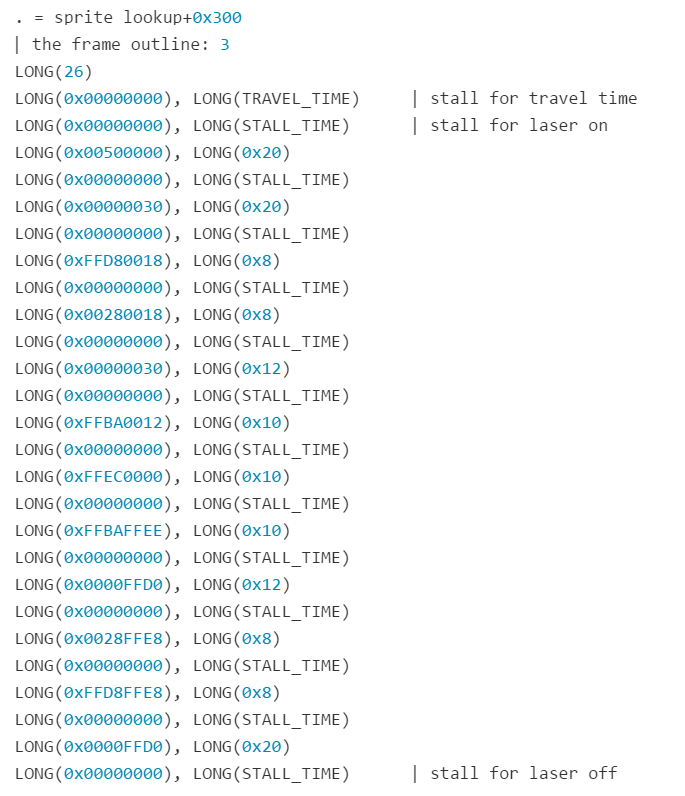
\includegraphics[width=0.75\textwidth]{sprite_lookup_laser}
\caption{The frame outline entry from the laser Beta's sprite lookup table.}
\end{center}
\end{figure}

Each sprite was broken up into line segments, and each line segment was broken up into sub-segments in order to not overdrive the galvos (which can only be driven a small distance at a time). The first item of each sprite (here "LONG(26)") is the number of line segments in that sprite. This is used as a countdown so the laser beta knows when it's reached the end of the sprite. The numbers in the left column describe x (most significant two bytes) and y (least significant two bytes) offsets, and the numbers in the right column are the number of times the corresponding offset is repeated. These offsets describe the length and direction of each sub-segment.

 To draw the sprite, each offset in the table is split into its x and y components, sign-extended, and added to the initial x and y location received from the physics beta; the initial location, which was registered, is then updated to store the current location. This new x-y point is then written to the galvos via the SPI module. This process is repeated with the same offset the specified number of times (drawing each sub-segment one at a time) until the end of the segment is reached; the next set of offsets is then loaded and the entire process is repeated until the segment counter runs out and the end of the sprite is reached.
 
Null offsets were inserted into the sprite table at the beginning and end to account for laser travel and power toggle time; null offsets were also added at sharp corners to counter the effects of the galvos' inertia.

\subsubsection{Galvanometers and DACs} \label{galvos}

The external hardware for the laser display—the DAC used to control the galvanometers, the laser, and the galvanometers themselves—were treated as memory-mapped peripherals and controlled simply by writing to and reading from the corresponding location in memory. Generating a coherent display on a laser projector, however, has a fair share of problems inherent to the hardware that must be solved. The two main problems were issues of inertia: the galvanometers are extremely slow compared to the 50MHz clock of the Beta, and driving them any faster than about 20kHz could break them; similarly, the laser has a not-insignificant power on and off time. These are some of the problems with commercial laser projection systems, as well: the inertia of the galvos tends to round out sharp corners, and the designer has to be careful of laser power during travels between sprites. These issues were accounted for in the sprite drawing process described above with the addition of "null offsets": the effects of these offsets can be clearly seen in the images below.

\begin{figure}[H]
\centering
\begin{minipage}{.5\textwidth}
  \captionsetup{width=0.8\textwidth}
  \centering
  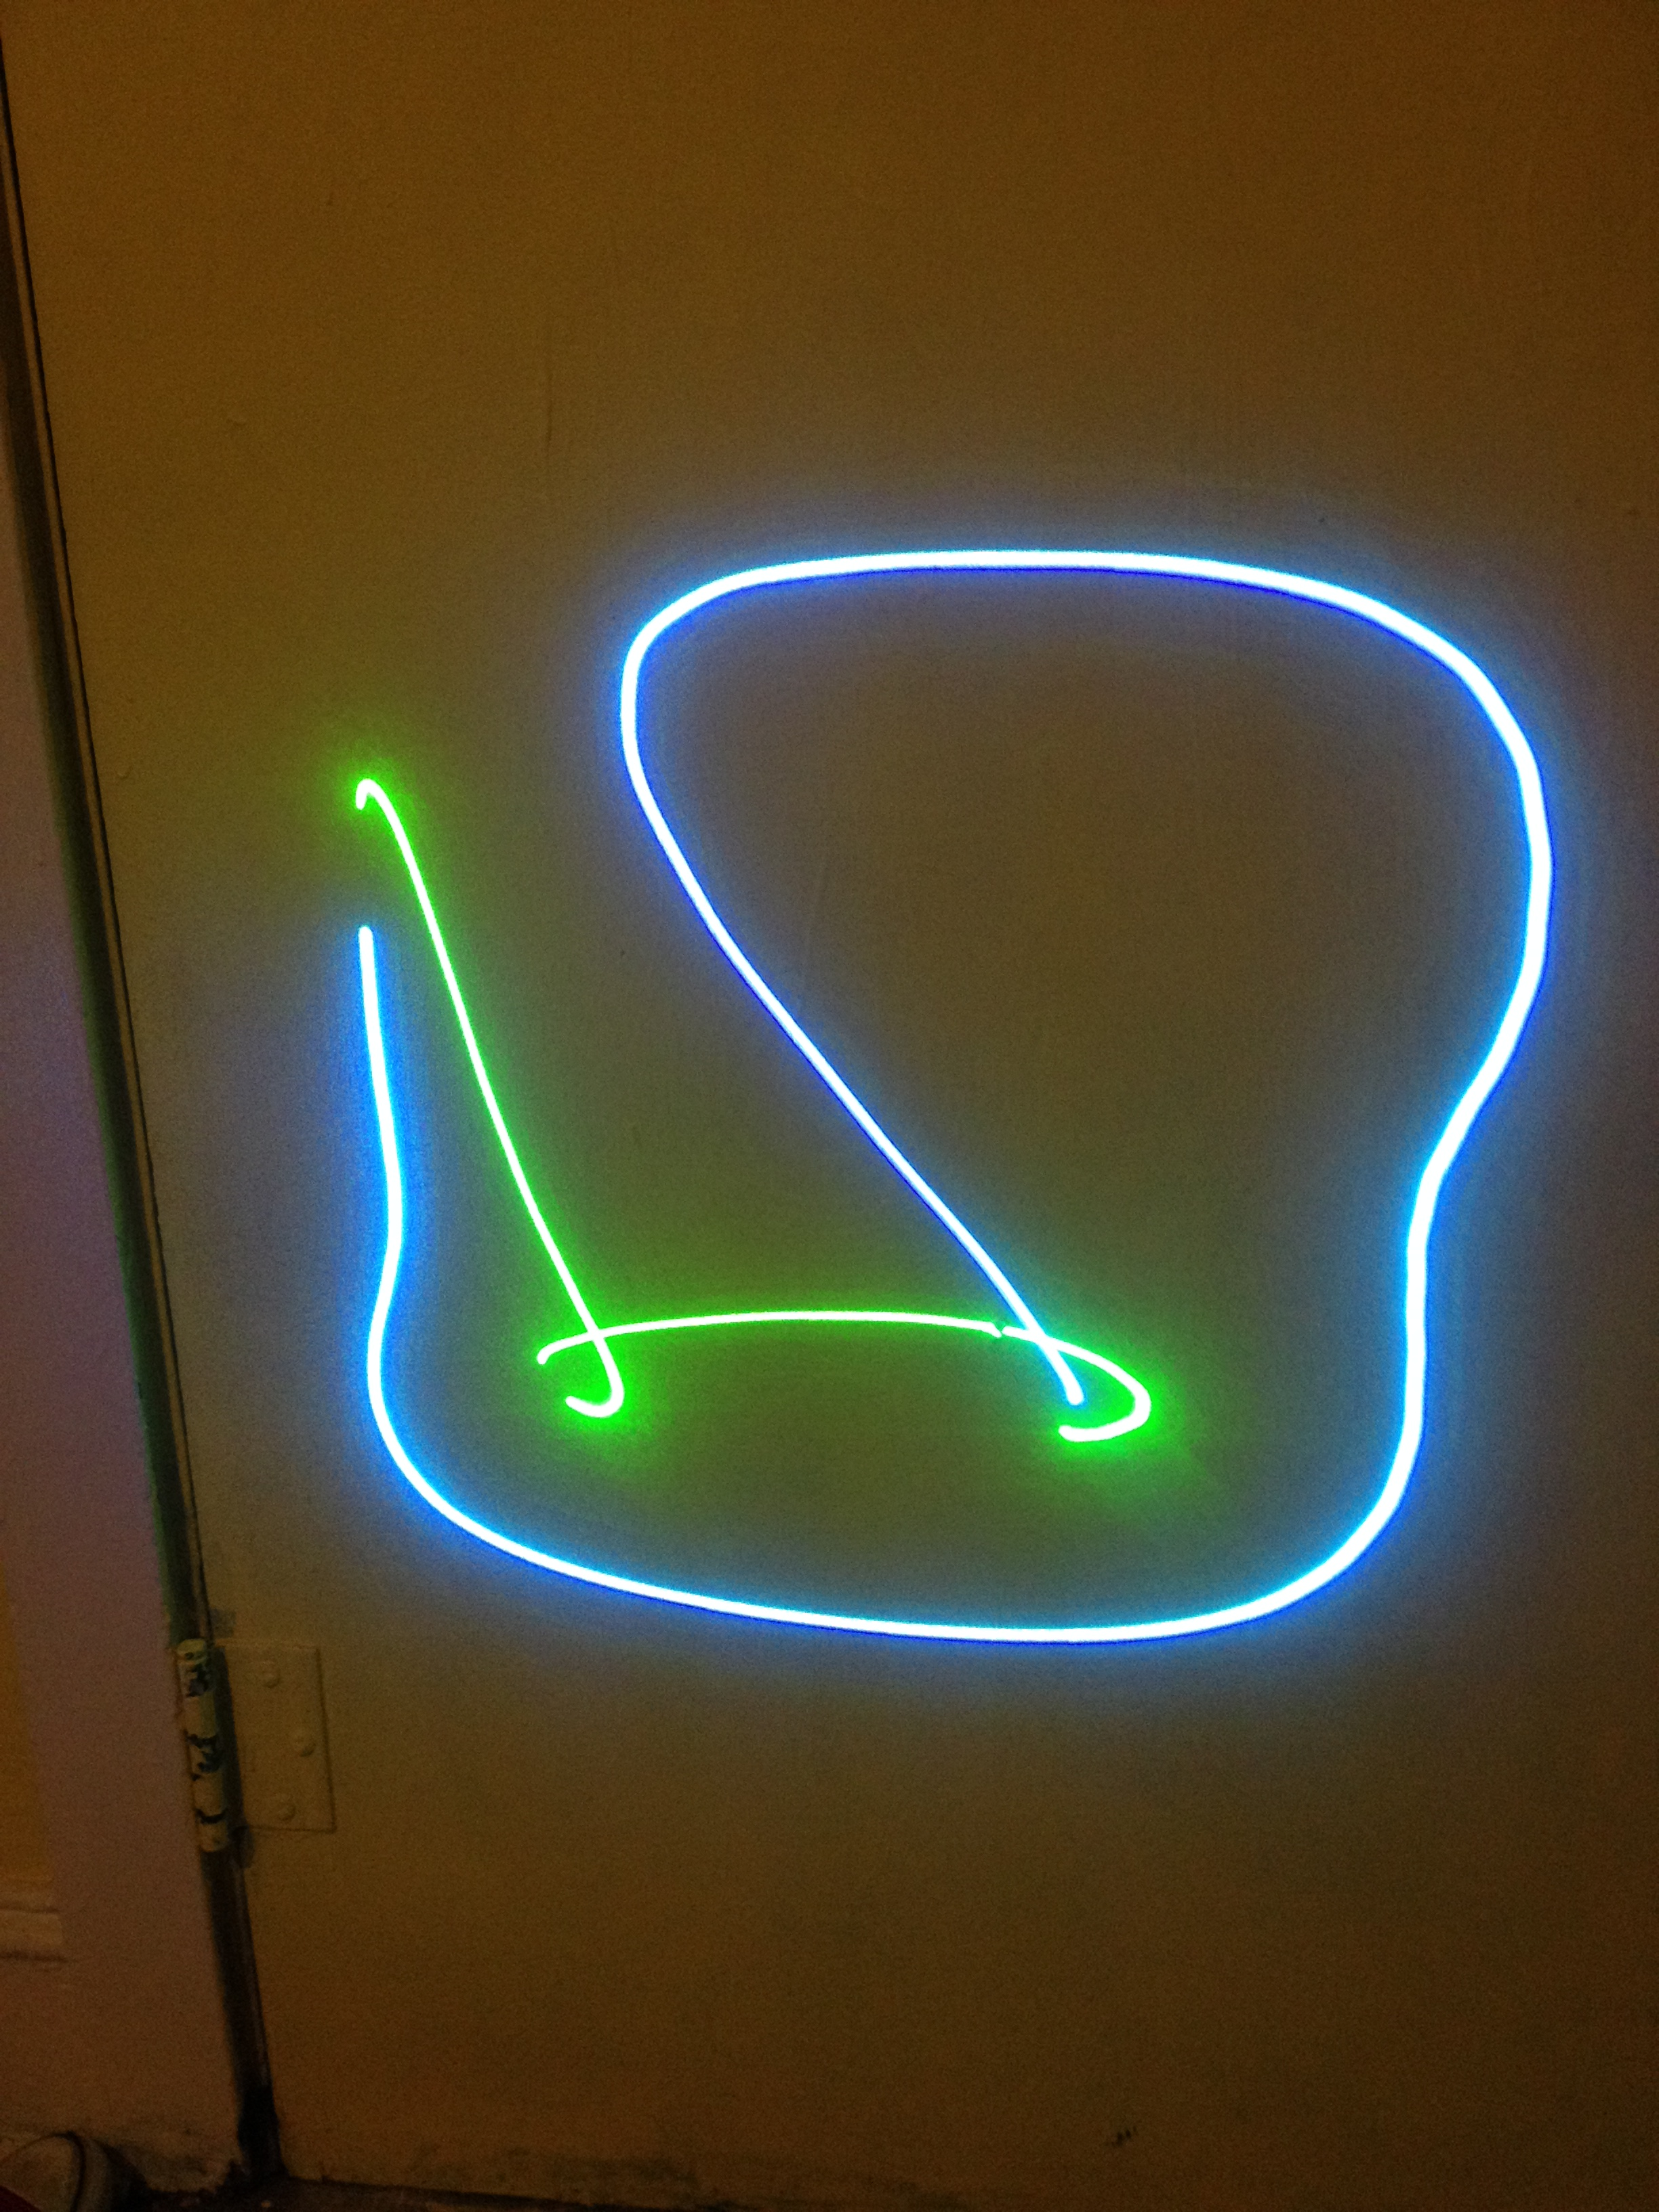
\includegraphics[width=.6\linewidth]{laser_loopy}
  \caption{The display without corner stalls or stalls for laser power.}
  \label{fig:loopy}
\end{minipage}%
\begin{minipage}{.5\textwidth}
  \captionsetup{width=0.8\textwidth}
  \centering
  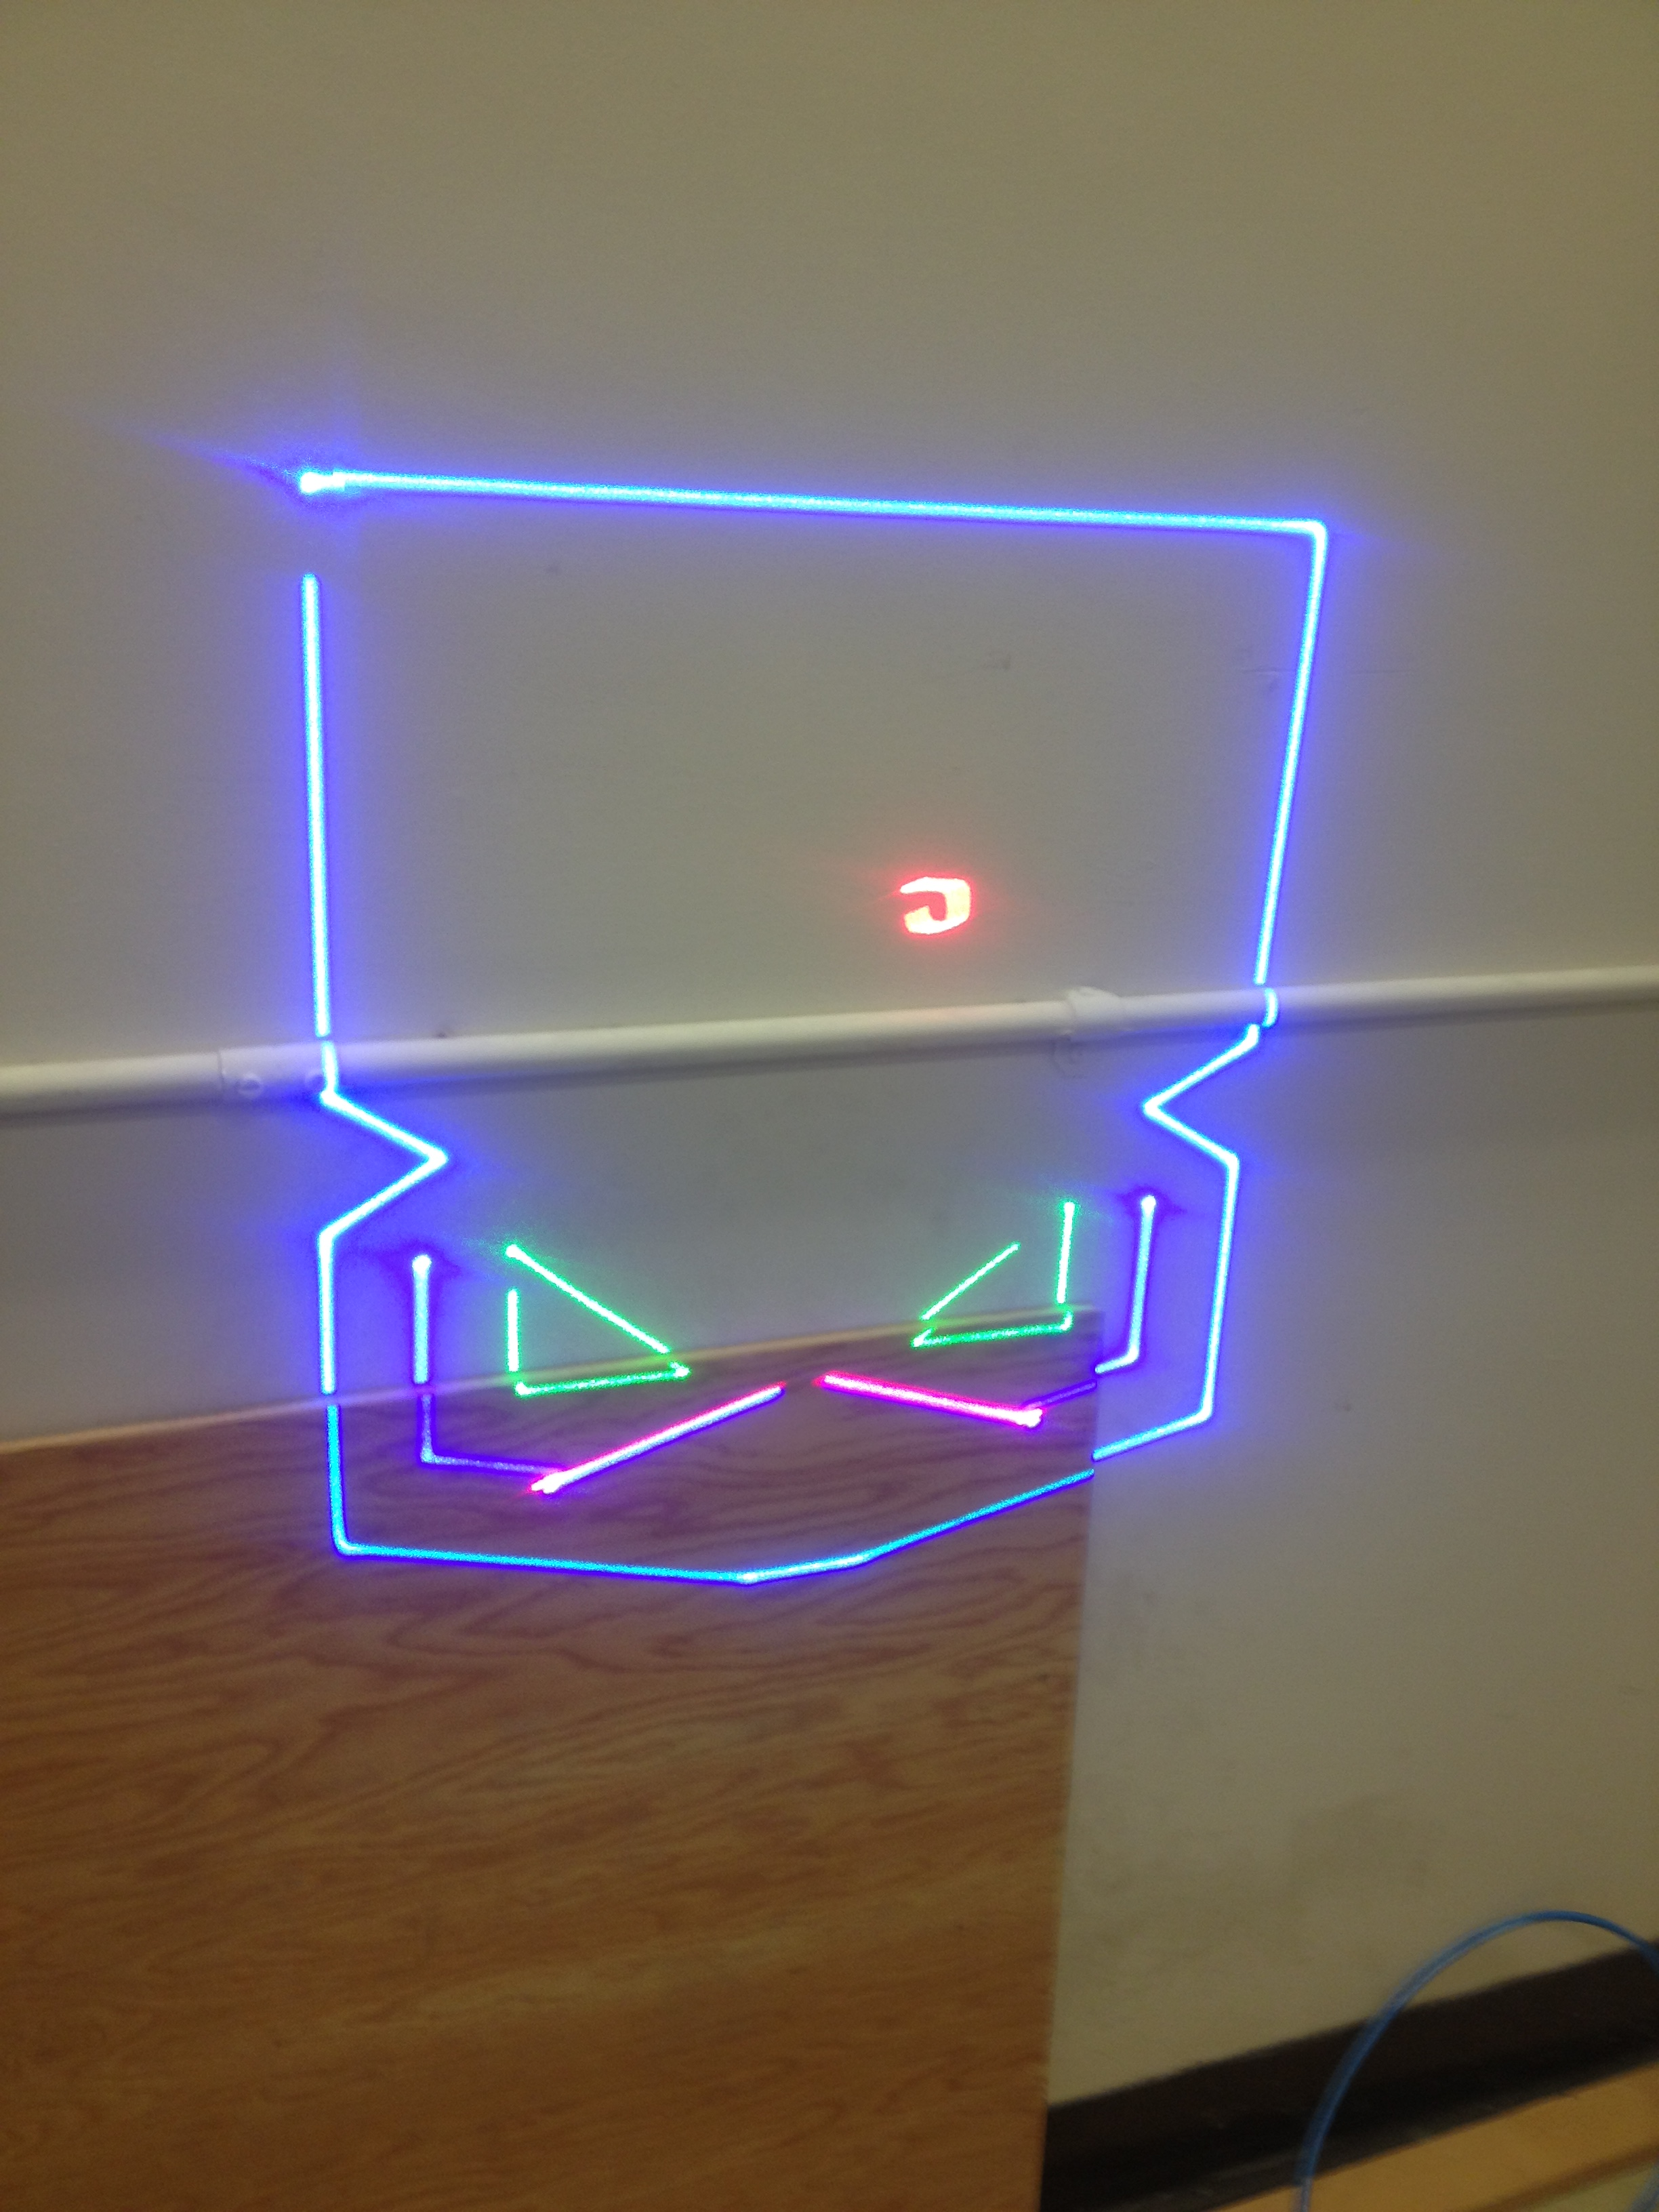
\includegraphics[width=.6\linewidth]{laser_success}
  \caption{Adding corner stalls to sharpen corners and wait periods for laser power toggle.}
\end{minipage}
\end{figure}

We also encountered less common issues, such as one of our first figures being rotated by 90$\degree$ because of a swapped pair of wires on the board. Additionally, an error in the schematic for the laser control board resulted in a limited rotation field for the galvos--the board couldn't drive negative voltage and so was clipping the reachable field to the lower right quadrant. This resulted in our first few tests being much smaller than expected given the values we were sending to the galvos. Coding bugs (like underflow and overflow) also became painfully obvious during laser display testing.

\begin{figure}[H]
\centering
\begin{minipage}{.5\textwidth}
  \captionsetup{width=0.8\textwidth}
  \centering
  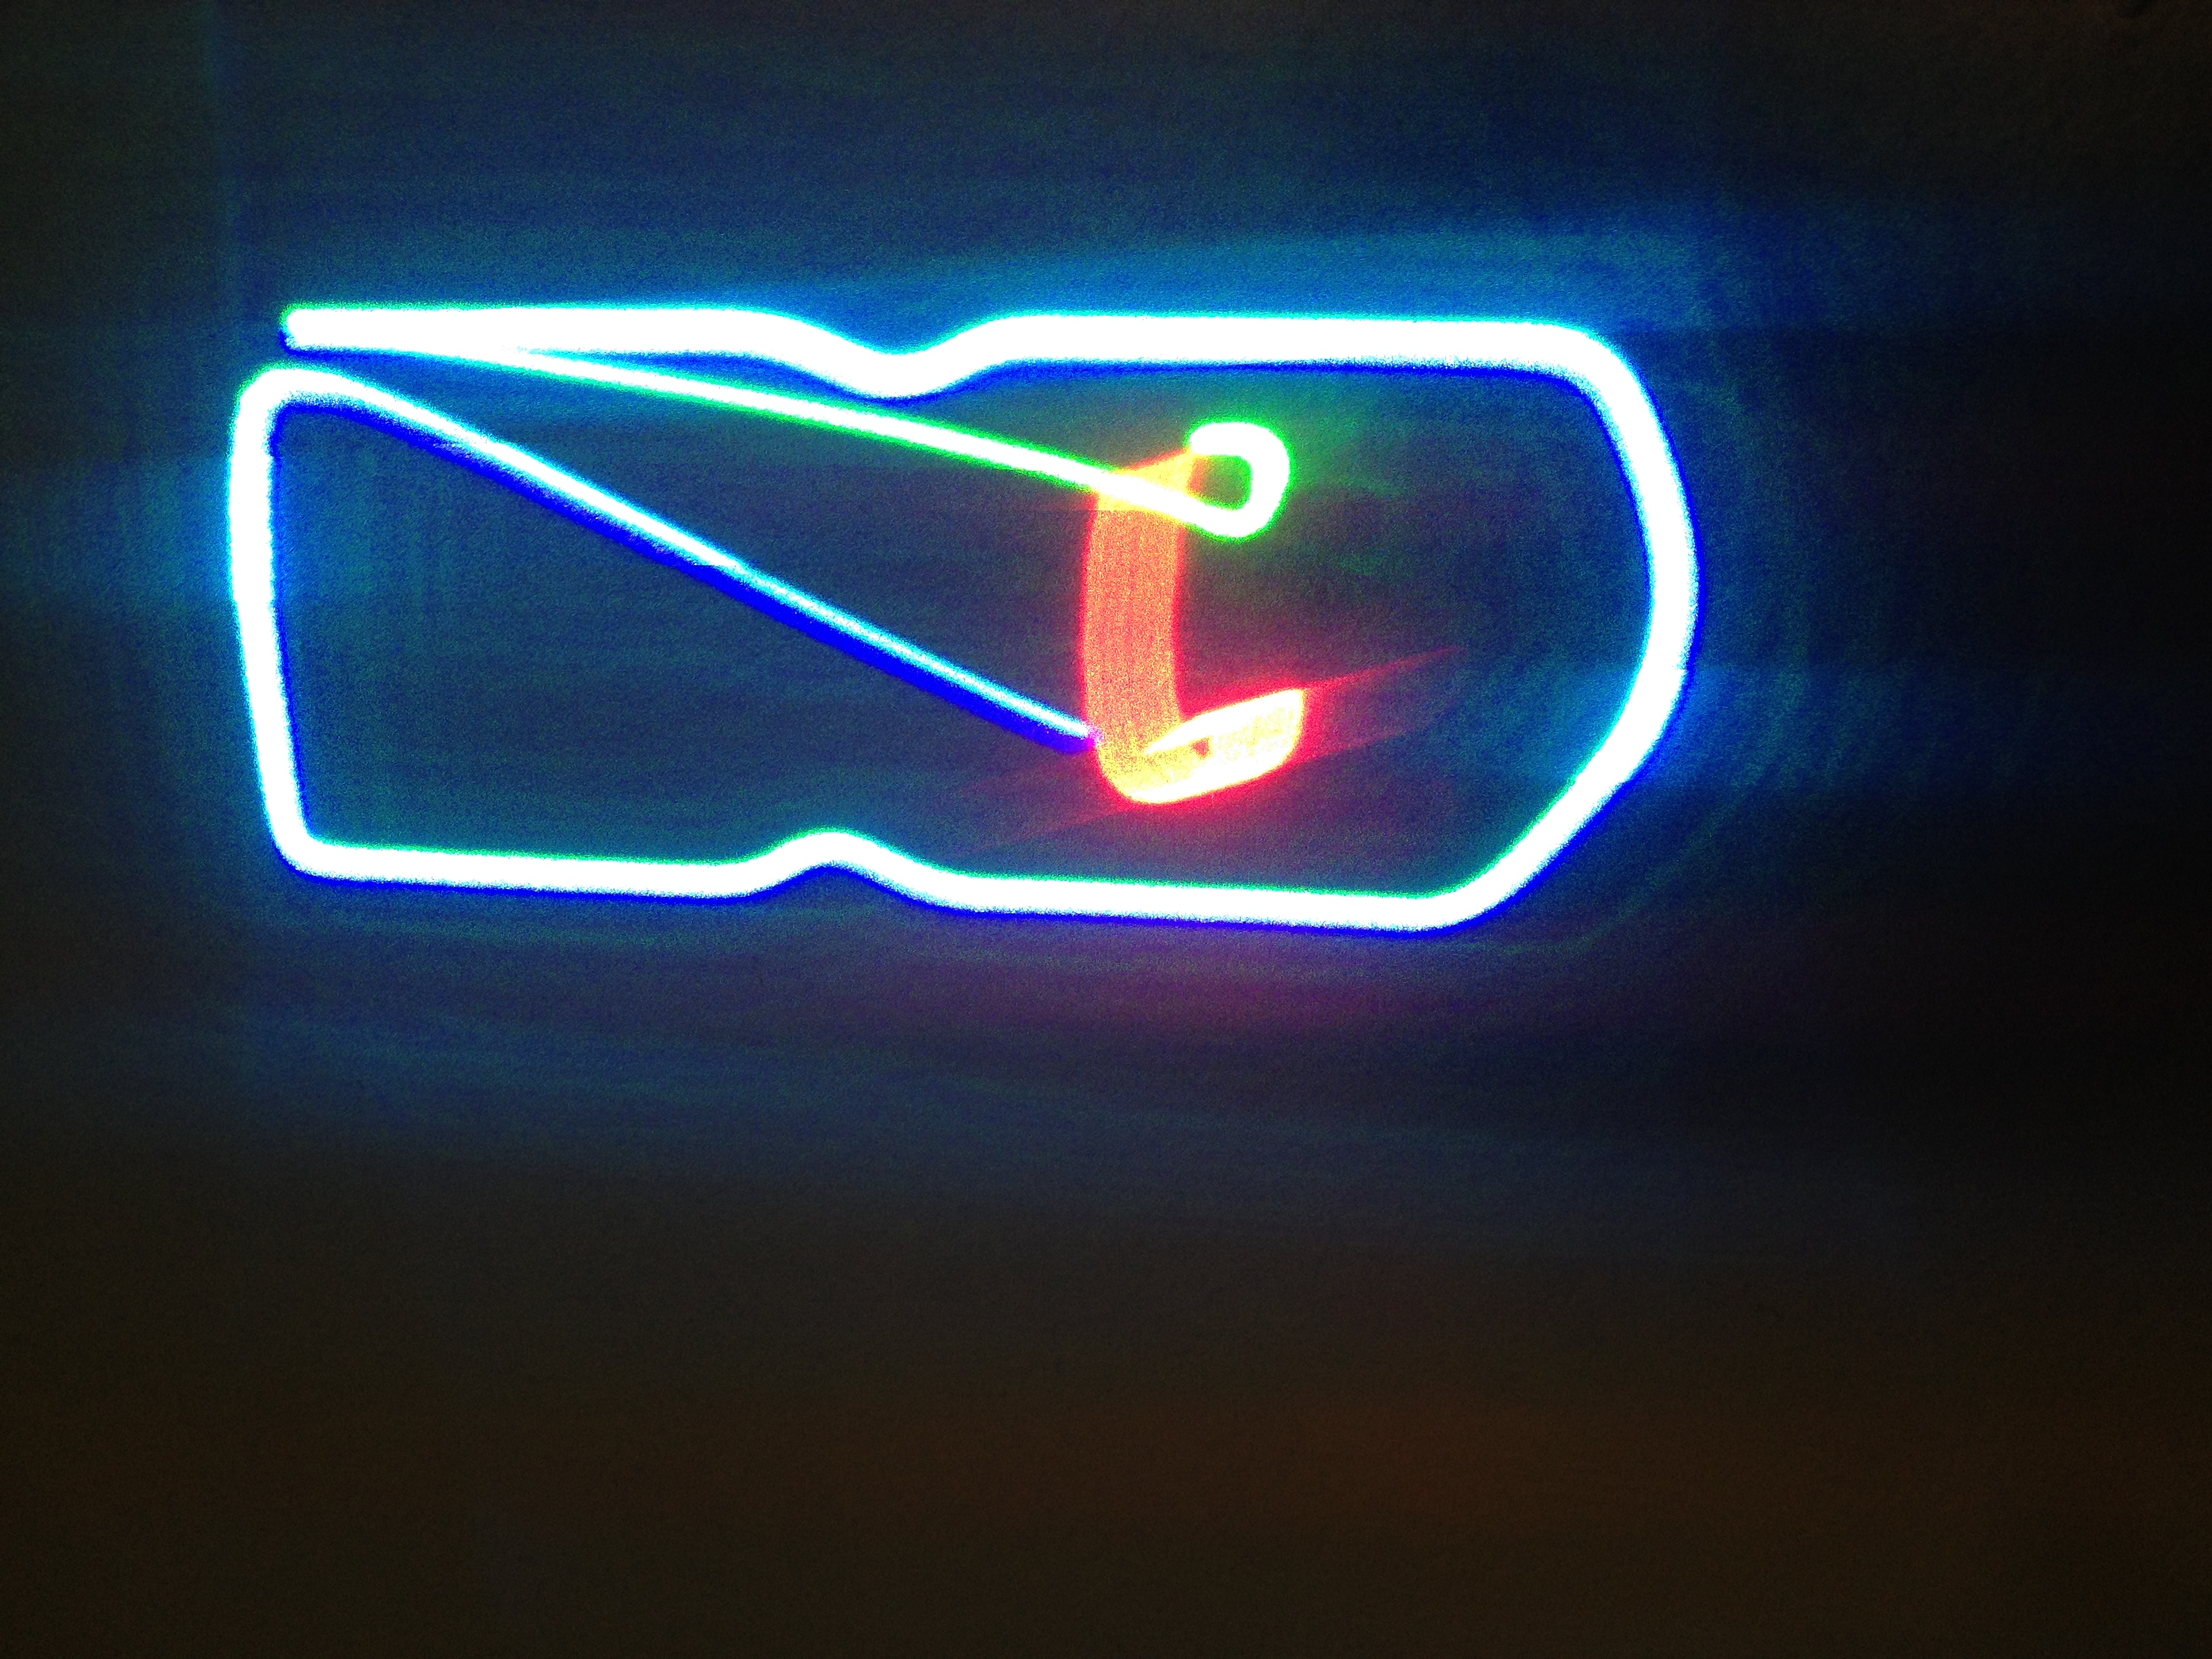
\includegraphics[height=2in]{laser_rotated}
  \caption{One of the first laser tests, both small and rotated.}
\end{minipage}%
\begin{minipage}{.5\textwidth}
  \captionsetup{width=0.8\textwidth}
  \centering
  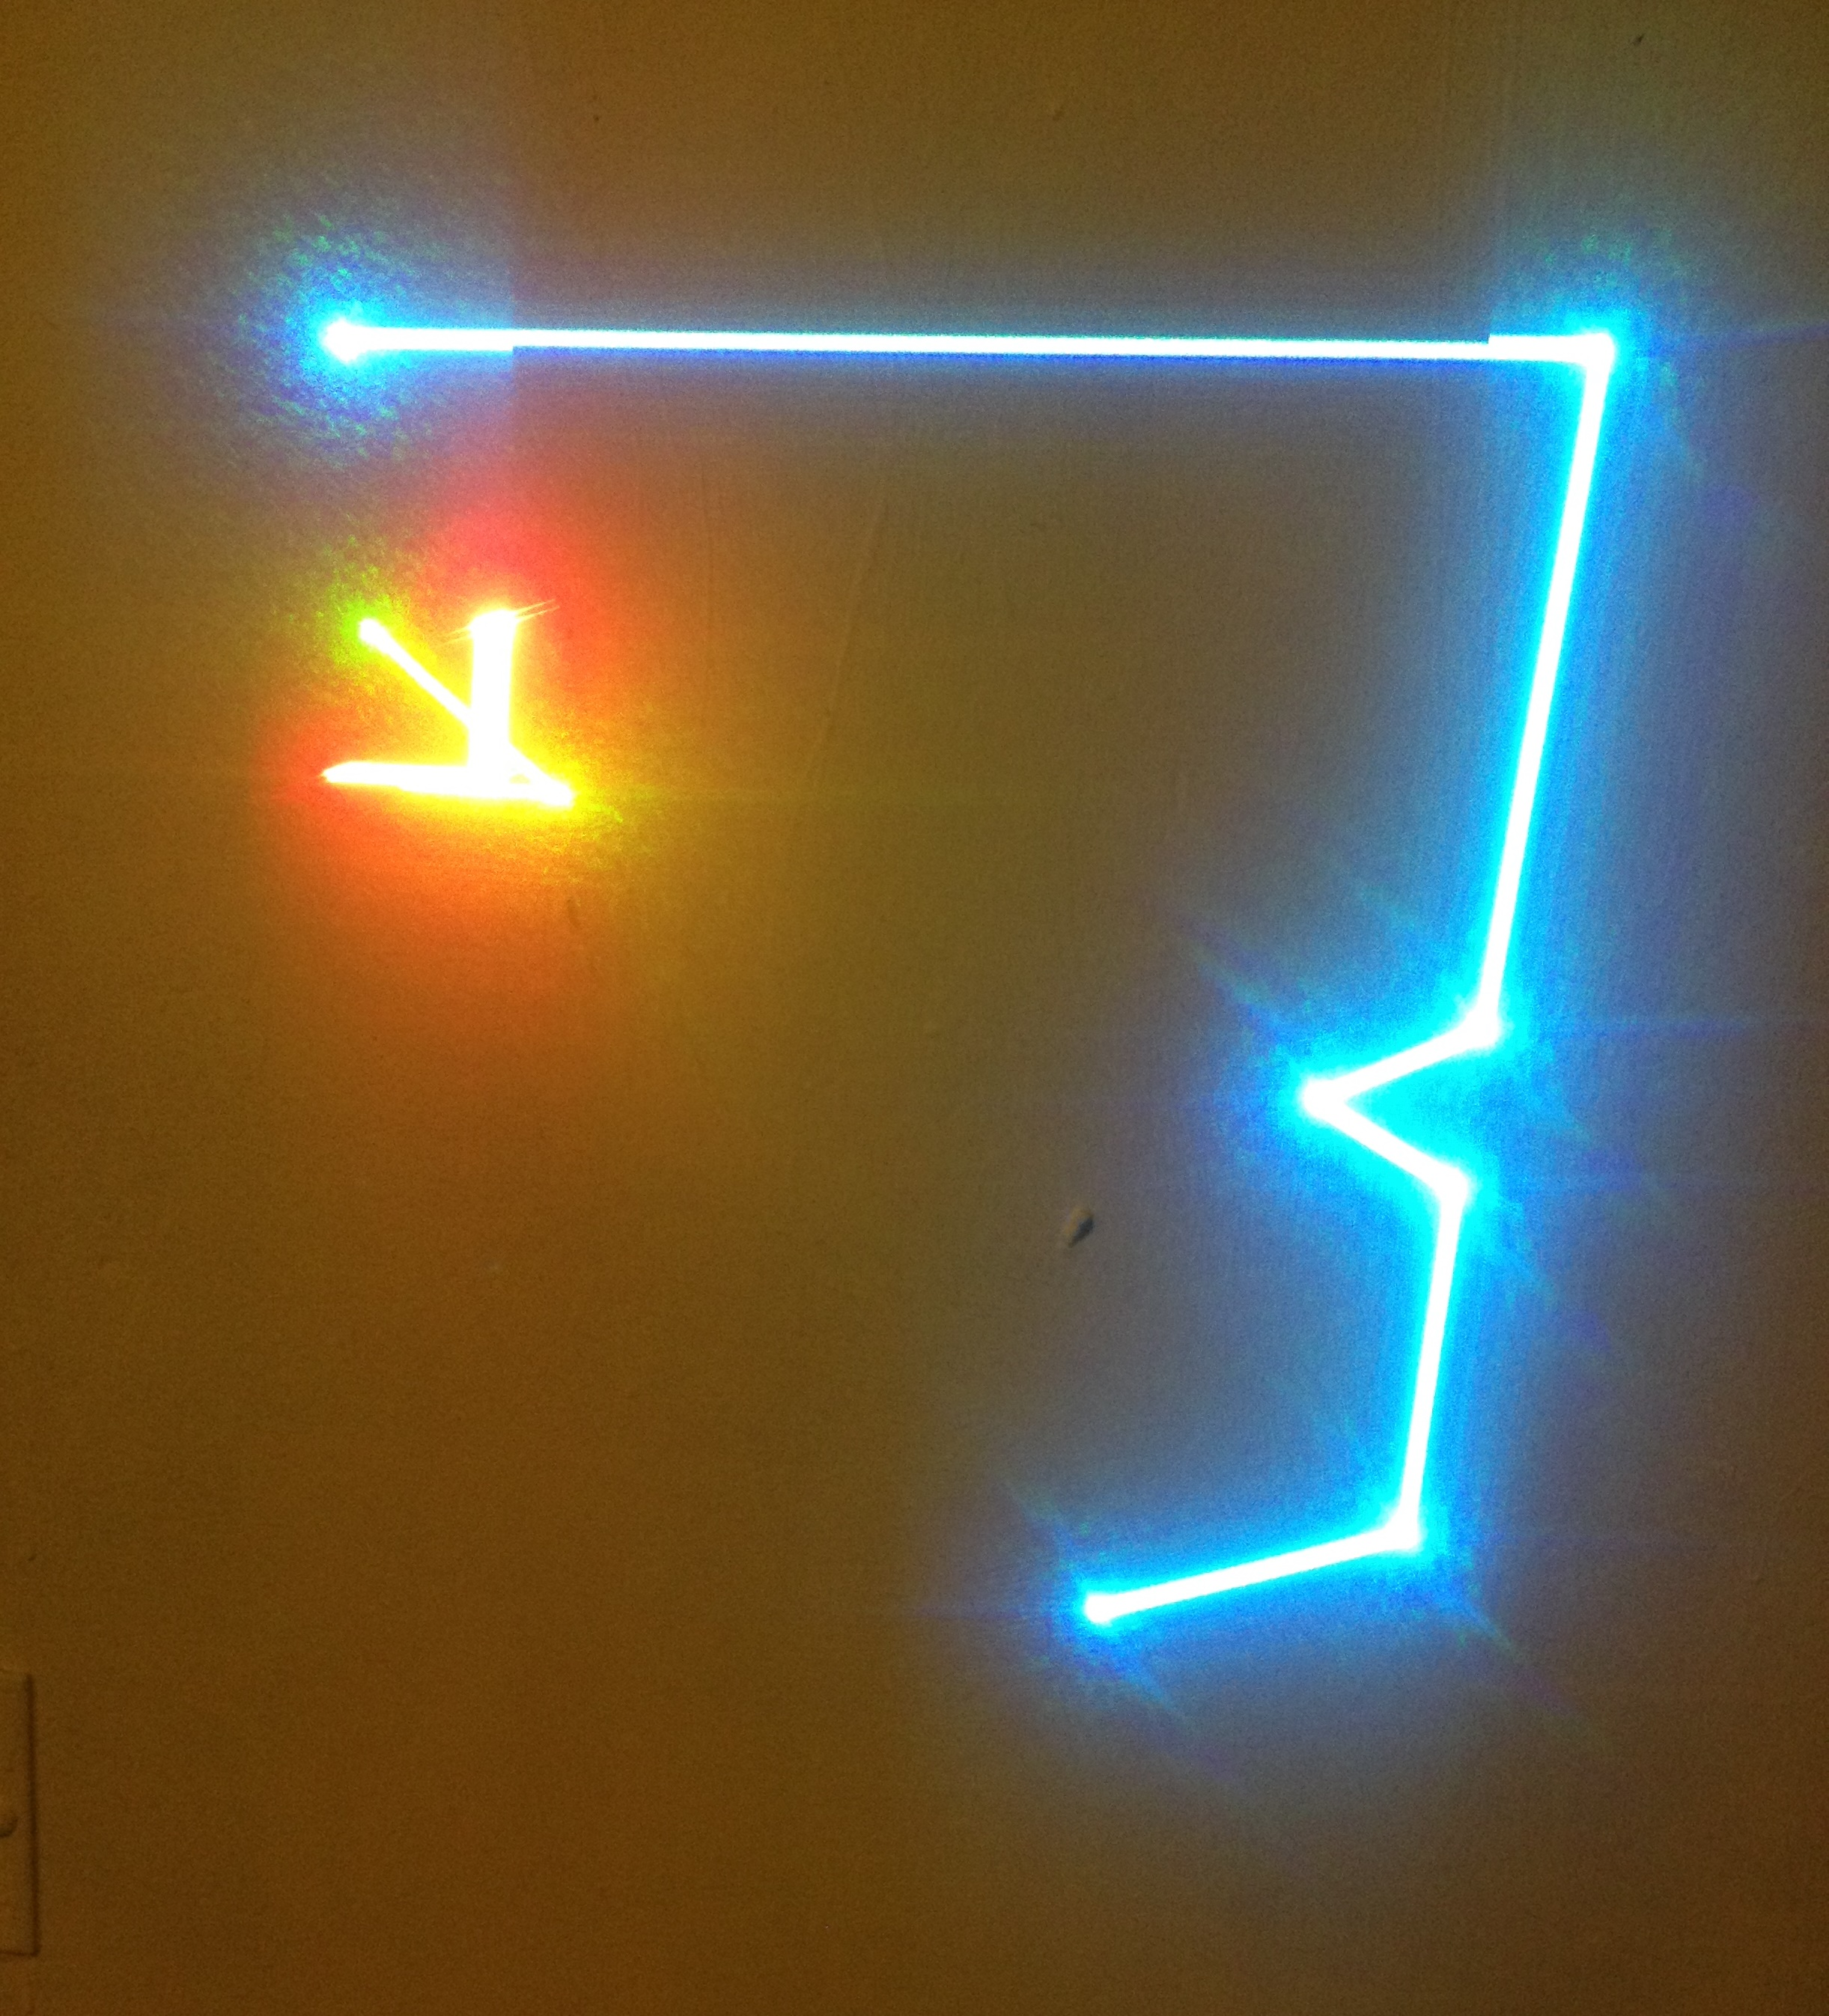
\includegraphics[height=2in]{laser_derp}
  \caption{An assembly bug resulting in the drawing of only half of a sprite.}
\end{minipage}
\end{figure}

\begin{figure}[H]
\centering
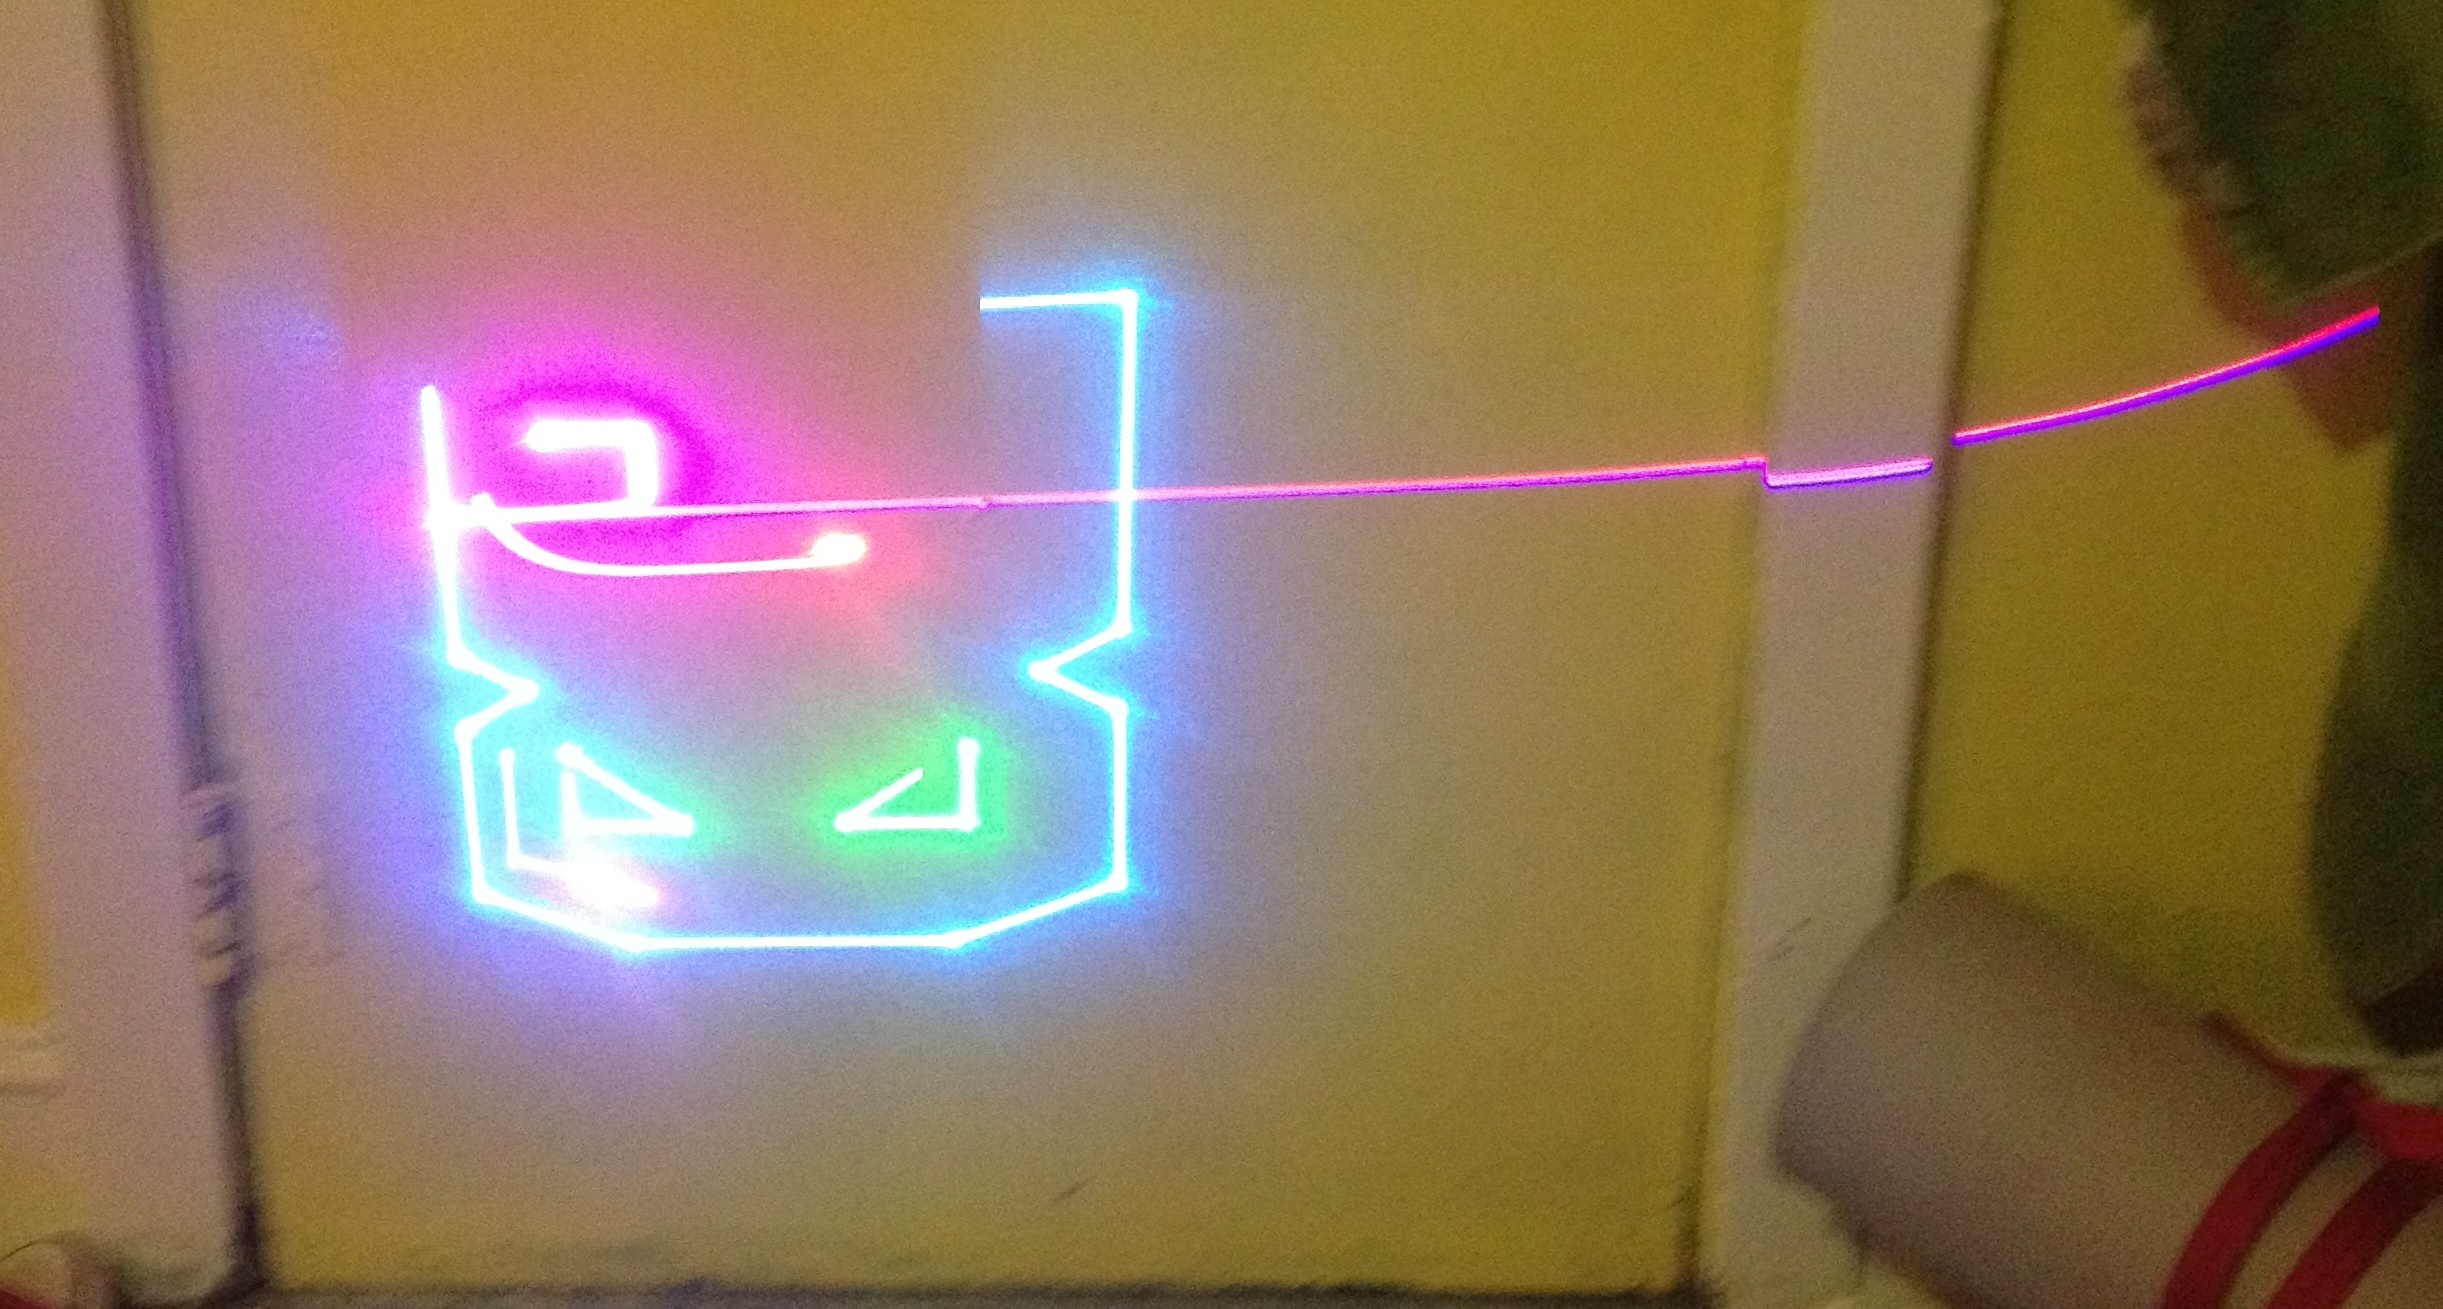
\includegraphics[width=0.5\textwidth]{laser_underflow}
\caption{Problematic register underflow causing the laser beam to shoot to the maximum extent of its range.}
\end{figure}

\end{document}